\documentclass[10pt,conference]{IEEEtran}

% --- Packages ---
\usepackage{cite}
\usepackage{amsmath,amssymb,amsfonts}
\usepackage{graphicx}
\usepackage{textcomp}
\usepackage{xcolor}
\usepackage{booktabs}
\usepackage{multirow}
\usepackage{url}
\usepackage{balance}
\usepackage{algorithm}
\usepackage{algorithmic}

% --- Project macros ---
\newcommand{\toolname}{VulnVersion}
\newcommand{\need}[1]{[\textit{#1}]}

\begin{document}

\title{From Patch to Affected Releases: Predicate-Guided Vulnerability-State Verification across Software Versions}

\author{Anonymous Authors}

\maketitle

\begin{abstract}
Identifying which released versions are affected by a disclosed vulnerability is essential for vulnerability management, dependency maintenance, and downstream risk assessment. Existing approaches often infer affected version ranges from advisory text, fixing commits, or vulnerability-inducing commits, but such interval-based reasoning is fragile under backports, release-branch divergence, refactorings, partial fixes, and vulnerability-preserving code movement. This paper formulates CVE affected-version identification as release-level vulnerability-state verification. Given a CVE fixing commit and a repository's release history, our key insight is that each release tag should be classified by verifying whether the root-cause vulnerability predicate still holds in that release, rather than by its position in a commit interval. We present VulnVersion, a predicate-guided approach that extracts root-cause anchors and vulnerability/fix predicates from patches, collects repository-local evidence across release tags, and produces tag-level vulnerability states through evidence aggregation and constrained LLM-assisted semantic judgment. We evaluate VulnVersion on a public benchmark for vulnerability-affected version identification and compare it against advisory-based, commit-range, SZZ-style, patch-similarity, and LLM-only baselines.
\end{abstract}

\begin{IEEEkeywords}
software vulnerability, affected-version identification, software evolution, program analysis, large language models
\end{IEEEkeywords}

\input{Sections/01_Introduction}
\section{Background and Problem Formulation}
\label{sec:background}

\subsection{Affected-Version Identification}

This paper studies the vulnerability-affected version identification task defined by the benchmark study of Chen et al.~\cite{howfar2025}. Given a reported vulnerability $c$, such as a CVE, a target project or repository $P$, a set of released versions or release tags $V=\{v_1,\ldots,v_n\}$, and patch evidence such as one or more fixing commits, the task is to identify the subset of releases in which the vulnerable logic remains present:
\[
V_{\mathit{aff}}(c,P) = \{v \in V \mid \mathit{vuln\_state}(c,P,v)=\mathsf{true}\}.
\]
Here $\mathit{vuln\_state}$ is a task-level predicate, not an assumed oracle. It names the conceptual release-level property that tag $v$ still contains the vulnerability condition associated with $c$. Later sections operationalize this property through repository evidence and branch-specific history reasoning.

The output is therefore a set of released versions, not a vulnerability-inducing commit, not a vulnerable function, and not a textual advisory range. This distinction is central to the benchmark study by Chen et al.: the evaluation treats exact recovery of the full affected-version set as a vulnerability-level objective, while also measuring partial correctness over individual CVE-version pairs~\cite{howfar2025}. A method can be useful at one granularity and still fail at the other. For example, predicting many truly affected tags may yield a reasonable version-level recall, but a single omitted affected tag makes the CVE-level exact set wrong.

The benchmark setting is also repository-grounded. The released-version universe is determined by project release tags, and the ground-truth labels are attached to those released versions. In this paper, we use the same task framing and benchmark family as Chen et al.: the goal is to predict \texttt{affected\_versions} for each CVE in the dataset, using repository and patch evidence rather than treating public advisory metadata as sufficient ground truth.

\subsection{From Fixing Patches to Vulnerability State}

A fixing patch is the most useful starting signal for this task, but it is not the answer. A commit that closes a CVE may contain the root-cause fix, supporting checks, error-handling changes, tests, documentation, refactoring, wrapper changes, formatting edits, or branch-specific backport adjustments. The patch also describes a transition from one repository state to another, whereas affected-version identification asks whether many released states still satisfy the vulnerable condition.

We use two conceptual predicates to separate these roles. A \emph{root-cause predicate} describes the condition that makes the vulnerability possible in a repository state, such as a missing bounds check, an unchecked object lifetime, an attacker-controlled value reaching a sensitive operation, or an invalid state transition. A \emph{fix predicate} describes the condition introduced or restored by the patch that prevents the vulnerability. Code presence alone may also be insufficient when the vulnerability depends on attacker-controlled inputs, trigger conditions, configuration, reachable sinks, or exploit preconditions. These attacker-relevant conditions should be preserved as structured evidence rather than only as unstructured prompt text. These predicates are conceptual objects in this section; the concrete extraction and checking procedures are deferred to Section~\ref{sec:approach}.

This predicate view prevents a common category error. The old side of a patch may provide a pre-fix anchor, but the anchor is only evidence about where to search. The new side of a patch may provide a fix predicate, but the absence of that new code in an old release does not automatically prove that the old release is vulnerable. A release is affected only when the root-cause predicate, under the relevant repository context, still holds in that release.

\subsection{Attacker Conditions and Vulnerability Evidence Graphs}

Affected-version identification cannot be reduced to code similarity, patch-line matching, or BIC localization. A vulnerable line matters only when the surrounding repository state still permits the vulnerable behavior. This state often depends on attacker-relevant conditions: attacker-controlled input, a trigger condition, an exploit precondition, a reachable sink, a missing guard, an unsafe state transition, or a security condition such as object lifetime, bounds, recursion, integer overflow, or a type invariant.

For this reason, a root-cause predicate is not just a code line. It should be tied to the vulnerable condition, the fix predicate or fix condition, source evidence, patch evidence, and the path or state constraint that makes the vulnerability relevant. The evidence may include a reachable sink, a missing guard, an unsafe state transition, a pre-fix anchor, or a history event that preserves or changes the condition. For affected-version identification, an attacker perspective does not mean proving a working exploit for every release. It means preserving the conditions under which the vulnerable behavior can be triggered, so that later history reconstruction does not confuse a syntactically similar line with a security-relevant state.

These relations are hard to preserve as flat prompt text. They are also easy to lose in a flat JSON record that lists evidence items without their roles. The evidence for one CVE can connect a CVE description, CWE category, fixing commit, patch hunk, pre-fix anchor, root-cause predicate, fix predicate, attacker condition, history event, and boundary event. A graph representation provides a structured substrate for these relations. In this limited sense, an attack-perspective knowledge graph is a way to organize attacker conditions and repository evidence, not a generic security ontology or an exploit proof. Its purpose is narrower: to keep evidence connected across the affected-version pipeline, from root-cause evidence to SZZ anchors, history events, boundary-event judgment, Git-DAG state propagation, and release tag projection.

\subsection{Why BIC Localization Is Insufficient}

SZZ-style methods locate bug-inducing commits (BICs) or vulnerability-inducing commits (VICs) by tracing from a fixing commit back through file history. This evidence is useful because the introduction of a vulnerable statement or state can bound where the vulnerability may have appeared. V-SZZ connects this idea to affected-version inference by mapping vulnerability-inducing commits to released version ranges~\cite{vszz2022}; later work improves commit localization through semantic analysis, LLM-assisted statement and candidate assessment, agentic repository search, and temporal knowledge-graph search~\cite{tcszz2024,llm4szz2025,agentszz2026,howwhyagents2026,beyondblame2026}.

However, a BIC or VIC is a history event, while an affected-version set is a projection over released repository states. Even a correct inducing commit does not by itself determine all affected releases. The method must still determine which branch-specific states reach official release tags, which branches received the fix, whether equivalent fixes exist without the same commit hash, and whether later code movement or partial reverts changed the vulnerability state.

The gap becomes larger in non-linear histories. A vulnerability may be introduced on one branch, fixed on another, backported to selected stable branches, or fixed through different commits in different release lines. Multi-fix CVEs and partial fixes further break the assumption that a single inducing commit and a single fixing commit define a closed linear interval. Therefore, BIC localization provides history evidence, but affected-version identification requires boundary-event judgment and branch-aware release projection.

\subsection{Tracing-Based and Matching-Based Evidence}

The benchmark study organizes existing affected-version tools into two evidence families~\cite{howfar2025}. Tracing-based methods start from fixing patches, select statements or hunks, trace them through history toward candidate inducing commits, and then infer affected versions from the resulting history range. Matching-based methods construct vulnerability signatures, patch signatures, or code representations and search historical versions for matching vulnerable logic.

Both families produce useful evidence, but neither evidence family is equivalent to complete affected-version reasoning. Tracing evidence can identify plausible historical events, yet it may be sensitive to statement selection, one-step blame assumptions, over-tracing, and weak cross-branch patch reuse. Matching evidence can detect code presence, yet it may be brittle under renaming, refactoring, minor syntactic edits, and semantically equivalent but syntactically different code.

The benchmark evaluation deliberately uses both vulnerability-level and version-level metrics because the two evidence families fail in different ways~\cite{howfar2025}. Tracing-based tools often preserve temporal context but can miss the true vulnerable condition when the selected patch lines are not root-cause lines. Matching-based tools can achieve high precision on exact or near-exact patterns but often lack semantic verification that a matched snippet still constitutes the vulnerability. For this reason, the present paper treats tracing and matching outputs as evidence sources rather than final affected-version decisions.

\subsection{History and Release Structure Challenges}

Affected-version identification is difficult because patch structure and release structure interact. Add-only patches are hard for deletion-dependent tracing because the patch introduces guards or checks without deleting the vulnerable old statement. Deleted-line or modified-line patches are easier to anchor, but the deleted text may still be an implementation symptom rather than the root cause. Multi-function and multi-file patches add unrelated edits, helper changes, tests, or refactoring noise, making it harder to decide which code elements should drive the affected-version judgment.

Branch and release structure adds another layer. Many projects maintain multiple release lines, and a CVE fix may be applied to each line through cherry-picks, backports, merge commits, or semantically equivalent commits. A branch may receive only part of a fix, may revert a fix, or may already contain a different mitigation. Consequently, the same CVE can correspond to several boundary events: the first commit that introduces the vulnerable state, the fixing commit on one branch, equivalent fixes on other branches, and prerequisite commits that make the vulnerability reachable.

Code evolution also weakens naive signature reasoning. A vulnerable function can be renamed, split, copied, moved across files, wrapped by a new API, or refactored while preserving the same vulnerable behavior. Conversely, a syntactically similar function can be safe because a guard, configuration constraint, type invariant, or control-flow condition changed. The release universe itself must also be explicit. Affected-version predictions are evaluated over official released versions or release tags, not arbitrary Git refs or every historical tag.

\subsection{Evidence-Gated Continual Adaptation}

Affected-version identification has repeated structure across CVEs. Cases from the same repository may share release branches, backport style, subsystem layout, parser code, or dependency code. Cases with the same CWE may share a root-cause pattern, such as bounds checks, object lifetime, recursion limits, integer overflow, or type confusion. Fixing commits may also share patch patterns, such as add-only guards, changed validation logic, changed error paths, or branch-specific backports.

These repeated structures can help later CVEs, but only as evidence. They can inform pre-fix anchor selection, candidate history event ranking, boundary-event judgment, branch-specific fix reasoning, and failure diagnosis. For example, a verified observation that one repository backports fixes through equivalent stable-branch commits can help rank future candidate fixes in that repository. A verified failure mode for add-only guard patches can help avoid relying only on deleted lines. In both cases, the reusable information is the inspected evidence and its provenance, not a model's unsupported memory of a prior answer.

Direct model memory is risky for this task. It may hallucinate a prior pattern, overfit to development cases, preserve a wrong prior, leak benchmark labels, or hide the source of an error. Continual adaptation is useful only if it is evidence-gated. A previous decision should not become reusable knowledge merely because a model produced it. It should become reusable only when the decision is linked to inspected repository evidence, a stable patch pattern, or a verified failure mode.

Evidence-gated memory should therefore keep provenance, link observations to repository, CWE, and patch-pattern evidence, and allow an observation to be invalidated or downgraded when later evidence contradicts it. It should also separate reusable evidence from ground-truth affected-version labels. In this paper, continual adaptation is a design requirement and a future ablation target unless supported by explicit experiments. It should act as a prior for history reconstruction, not as the final affected-version decision.

\subsection{Problem Statement}

The problem studied in this paper is: given a CVE $c$, its fixing commit family $F_c$, a target repository $P$, and the official release-tag universe $V$, identify all and only release tags in $V$ whose repository states satisfy the root-cause vulnerability predicate for $c$. Here, $F_c$ denotes one or more fixing commits associated with the CVE, including branch-specific or equivalent fixes when such evidence is available. The expected output is a set of affected release tags, together with evidence and uncertainty records that explain how the prediction was derived.

This formulation deliberately excludes several adjacent tasks. It is not exploit generation and does not attempt to prove runtime exploitability for every released tag. It is not merely advisory normalization because advisory ranges can be incomplete, stale, or inconsistent with repository history. It is not only BIC or VIC localization because inducing commits are history events rather than release-level exposure labels. It is also not only vulnerable-code clone detection because code similarity is evidence, not a vulnerability-state verdict.

We describe the repository history as a Git directed acyclic graph (Git DAG). A \emph{history event} is a commit-level change that may introduce, remove, preserve, or transform part of the vulnerability condition. A \emph{boundary event} is a history event that changes the vulnerability state for a branch or release line. A \emph{release tag projection} maps these branch-specific vulnerability states onto the official release-tag universe. These definitions provide the vocabulary needed by the later method section without committing this section to a particular algorithm.

\subsection{Requirements for a Robust Solution}

The preceding formulation implies that an effective solution must be root-cause-grounded. It must distinguish vulnerability-relevant evidence from incidental patch edits, and it must represent both the vulnerable condition and the fixing condition before projecting branch-specific states to release tags. Without this separation, a method can confuse a wrapper change, a test update, or a backport artifact with the actual security state.

The solution must also be evidence-constrained. Pre-fix anchors, history events, and boundary events should be accepted only with repository evidence that can be inspected later. In particular, the method should separate the judgment that a candidate history event is relevant from the projection that converts branch-specific states into affected release tags. This separation is necessary because a candidate commit can be useful evidence without being the final affected-version boundary.

Finally, the solution must be branch-specific and auditable. It should reason over the Git DAG, release lines, backports, equivalent fixes, and official release tags rather than assuming a single linear version order. If LLMs or agents are used for semantic judgment, their role should be bounded and accountable: prompts, evidence inputs, uncertainty, failures, and decision artifacts must be recorded so that affected-version predictions can be inspected, debugged, and evaluated under the benchmark metrics. A robust solution should also support evidence-gated accumulation of repeated failures and verified history-event decisions as reusable repository, CWE, and patch-pattern evidence. Such memory must be auditable, not free-form model memory.

\section{Motivating Example}
\label{sec:motivating}

% TODO: Write motivating example showing why interval-based reasoning fails under backports, branch divergence, refactoring, and add-only fixes. Illustrate with a concrete CVE case.

\section{\toolname Approach}
\label{sec:approach}

This section describes the current high-level design of \toolname. It is intentionally written as a structured placeholder: it captures the design choices that are already supported by the local SystemDesign documents, while leaving implementation details, optimization choices, and final algorithmic claims as \need{NEEDS METHOD DETAIL}.

\subsection{Overview}
\toolname takes as input a CVE record, the target repository, the fixing commit family, release tags, and optional CVE context such as NVD description or advisory text. It outputs a predicted set of affected release tags. The framework is organized into three stages:
\begin{enumerate}[leftmargin=*]
  \item \textbf{Step1: fix-family and patch semantic filtering.} Parse fixing commits, extract changed files and hunks, classify commit-level and chunk-level roles, and produce patch semantics for later reasoning.
  \item \textbf{Step2: root-cause vulnerability evidence extraction.} Convert patch semantics and CVE context into root-cause-level evidence, including vulnerable sequences, fix guards, scope constraints, and evidence risks.
  \item \textbf{Step3: boundary-event reconstruction and release projection.} Build release-line structure, judge boundary events, propagate vulnerability state through the Git DAG, and project affected states to release tags.
\end{enumerate}

The corpus synthesis suggests a design rule that should be preserved as the method matures: deterministic evidence preparation should reduce the search space before expensive semantic judgment. FIRE, MOVERY, ReDeBug, V1SCAN, VULTURE, and VUDDY all use staged filtering or indexing to make vulnerability search scalable~\cite{fire2024,movery2022,redebug2012,v1scan2023,vulture2025,vuddy2017}; AgentSZZ and related agent papers show that scoped tool interfaces and context compression are important for keeping LLM-based repository investigation tractable~\cite{agentszz2026,howwhyagents2026}. \toolname adopts this as a paper-level boundary: semantic judgment should be scoped to evidence-backed boundary events, while Git-DAG state propagation and release-tag projection remain deterministic.


\begin{figure*}[t]
  \centering
  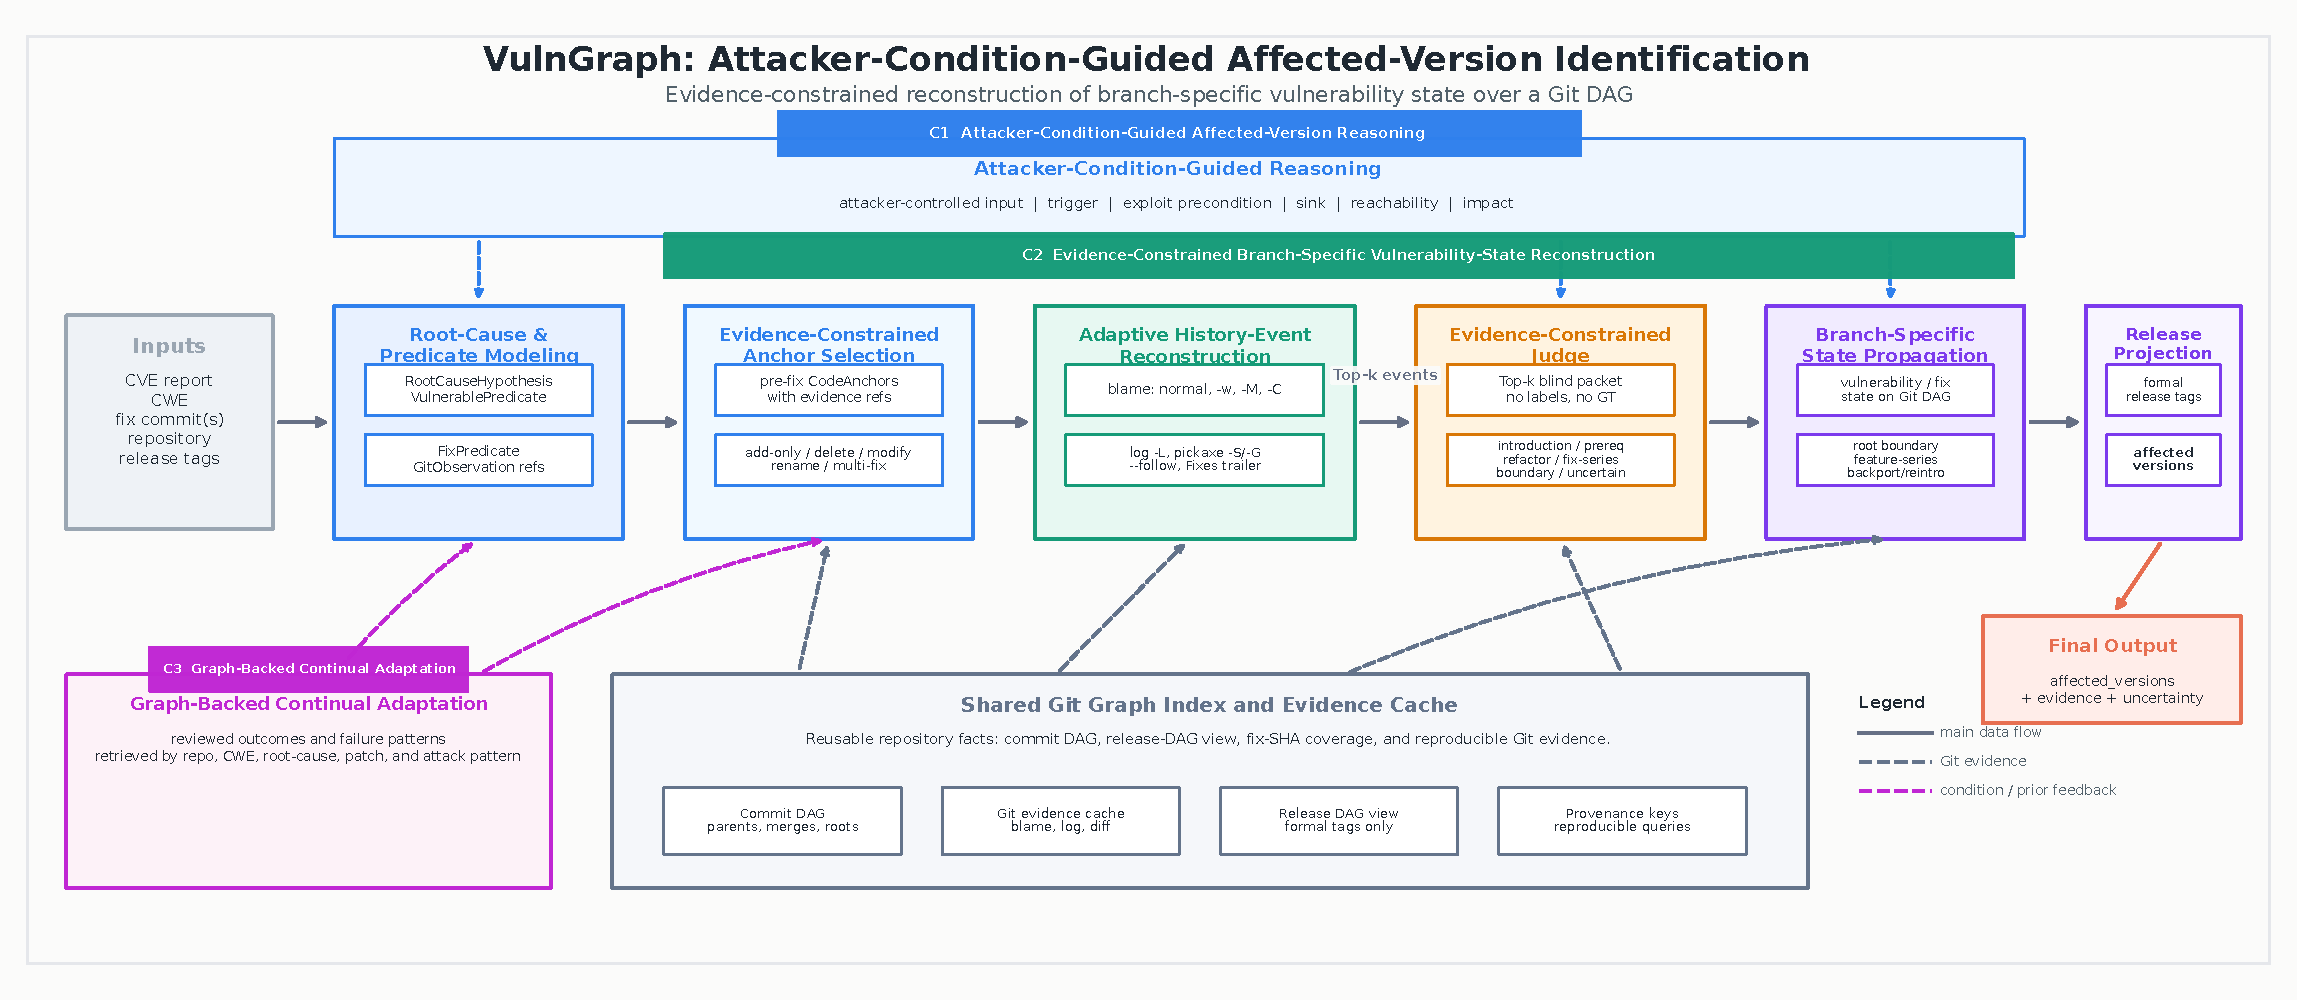
\includegraphics[width=\textwidth]{Figures/fig_vulngraph_overview.pdf}
  \caption{Overview of VulnGraph.}
  \label{fig:overview}
\end{figure*}

\subsection{Step1: Fix-Family Semantic Filtering}

The first stage exists because a CVE may map to multiple fixing commits and because each fixing commit may contain irrelevant hunks. The local design document records that the baseline dataset contains 1,128 CVEs and 1,542 patches, with 68 multi-commit CVEs after local flattening. It also records 4,783 patch chunks across the local dataset processing artifacts. These figures should be rechecked before camera-ready use \need{NEEDS EVIDENCE}.

Step1 is designed to output structured artifacts such as \texttt{fix\_family\_semantics.json}, \texttt{commit\_semantics.jsonl}, \texttt{chunk\_semantics.jsonl}, and \texttt{patch\_semantics.json}. Its role is not to decide affected versions. Instead, it provides clean, typed, and source-referenced patch evidence to Step2. In particular, Step1 should distinguish primary fixes from supporting fixes, contextual changes, tests, documentation, wrapper commits, and refactoring noise.

\subsection{Step2: Root-Cause-Level Evidence}

Step2 extracts a root-cause-level vulnerability existence theorem, abbreviated as VET in the design documents. The intended VET representation separates five concepts:
\[
\Theta = \langle S, V, F, G, C \rangle
\]
where $S$ is the vulnerability scope, $V$ is vulnerable evidence, $F$ is fix evidence, $G$ is guard or applicability constraints, and $C$ is the certificate policy. This representation is still a design placeholder \need{NEEDS METHOD DETAIL}, but it encodes an important boundary: touched files and changed lines are not automatically root-cause evidence.

Step2 should output artifacts such as \texttt{root\_cause\_vet.json}, \texttt{vet\_evidence\_graph.json}, \texttt{vet\_admission\_input.json}, and a compatibility \texttt{rci.json}. These artifacts provide the evidence packet used by Step3 for prioritizing boundary-event reconstruction.

This design is motivated by repeated warnings across the reference corpus: patch signatures, deleted lines, and cloned functions are useful evidence, but none of them alone proves that the vulnerability condition holds in a released version~\cite{vszz2022,redebug2012,vuddy2017,movery2022,vercation2026}. The VET artifact is therefore meant to make the required vulnerable condition explicit before boundary events are judged.

\subsection{Step3: Boundary Reconstruction and Release Projection}

Step3 is responsible for affected-version identification. The current main path is: fixing commits, candidate history events, boundary-event judgment, Git-DAG state propagation, and release-tag projection.
The semantic-judgment boundary is explicit: judgment is applied to candidate boundary events, while the release-line graph and release-tag projection are handled by deterministic repository analysis.

This separation is central to \toolname. Deterministic Git-DAG state propagation keeps the method auditable and cost-aware; semantic judgment is reserved for cases where boundary evidence must be interpreted. The final Step3 design still requires experimental validation before it can be presented as a complete algorithm \need{NEEDS EXPERIMENT}.

\subsection{Expected Agent Interface}

The planned semantic-judgment interface is deliberately narrow. For each candidate boundary event, the model receives scoped evidence derived from Step1 and Step2, repository snippets around the event, and a required output schema containing a selected, rejected, or uncertain judgment plus evidence references. Inspired by agentic SZZ evaluations~\cite{agentszz2026,howwhyagents2026}, \toolname should log token usage, tool calls, latency, and failure modes for every judgment. The exact prompt, tool API, and judgment schema remain \need{NEEDS METHOD DETAIL}.

\subsection{Memory and Self-Evolution Hooks}

The broader SystemDesign materials describe typed memory, verifier-gated skill evolution, and artifact promotion as future capabilities. In this draft, these are not claimed as completed experimental components. They are positioned as optional design hooks: failed boundary judgments may become failure memories, repeated repair procedures may become procedural memories, and stable verified patterns may eventually be compiled into deterministic artifacts. Any final claim about these mechanisms requires implementation and ablation evidence \need{NEEDS EXPERIMENT}.

\section{Implementation}
\label{sec:implementation}

% TODO: Describe the implementation of VulnVersion. Cover the three-stage pipeline, toolchain, repository interfaces, LLM/agent integration, and key engineering decisions.

\section{Evaluation Design}
\label{sec:evaluation}

This section specifies the planned evaluation. It does not report final \toolname results. All missing results are explicitly marked.

\subsection{Dataset}

The main dataset will be the benchmark used by ``Vulnerability-Affected Versions Identification: How Far Are We?''~\cite{howfar2025}. The local reference analysis states that the benchmark contains 1,128 C/C++ vulnerabilities from nine open-source projects and 132 vulnerability types. Exact project-level table values and patch-type counts must be verified against repaired tables before final use \need{NEEDS TABLE REPAIR}. The dataset is selected because it is directly aligned with our target problem: given CVEs and patch commits, identify affected release versions.

\subsection{Baselines}

We will compare against the baselines organized in the benchmark study:
\begin{itemize}[leftmargin=*]
  \item \textbf{Tracing-based:} VCCFinder~\cite{vccfinder2015}, V-SZZ~\cite{vszz2022}, Lifetime~\cite{lifetime2021}, SEM-SZZ~\cite{semszz2024}, TC-SZZ~\cite{tcszz2024}, and LLM4SZZ~\cite{llm4szz2025}.
  \item \textbf{Matching-based:} ReDeBug~\cite{redebug2012}, VUDDY~\cite{vuddy2017}, MOVERY~\cite{movery2022}, V1SCAN~\cite{v1scan2023}, FIRE~\cite{fire2024}, and VULTURE~\cite{vulture2025}.
\end{itemize}

If official runnable artifacts are unavailable or inconsistent, we will report whether baseline values are taken from the paper table or reproduced locally. No reproduced baseline claim will be made until scripts, data, and environment are verified \need{NEEDS ARTIFACT}.

\subsection{Metrics}

We follow the metric structure extracted from the baseline and related papers:
\begin{itemize}[leftmargin=*]
  \item \textbf{CVE-level Accuracy:} the fraction of CVEs for which the predicted affected-version set exactly equals the ground truth set.
  \item \textbf{CVE-level No-Miss Ratio:} the fraction of CVEs for which all ground-truth affected versions are included in the prediction.
  \item \textbf{Version-level Precision/Recall/F1:} flattened version-level metrics over all CVE-version pairs.
\item \textbf{Resource metrics:} average time, input tokens, output tokens, total tokens, cost, agent calls, candidate boundary events, and execution failure rate for \toolname \need{NEEDS EXPERIMENT}.
  \item \textbf{Manual-workload and lower-bound metrics:} if complete FN validation is infeasible for some cases, we will report conservative lower-bound recall and manual inspection counts, following the evaluation style of developer-log based affected-version work~\cite{tdsc2024}.
\end{itemize}

% \input{tables/evaluation_metrics}  % TODO: create this table file

\subsection{Research Questions}

\textbf{RQ1: Overall effectiveness.} How accurately does \toolname identify affected versions compared with tracing-based and matching-based baselines? We will report CVE-level Accuracy, CVE-level NMR, and version-level precision/recall/F1. Result table: \need{NEEDS EXPERIMENT}.

\textbf{RQ2: Robustness across patch and repository conditions.} How does performance vary across add-only, delete-only, mixed patches, single-file and multi-file patches, and single-branch versus multi-branch settings? Subset definitions will follow the benchmark where available. Result table: \need{NEEDS EXPERIMENT}.

\textbf{RQ3: Contribution of each \toolname stage.} What is the effect of patch-family filtering, root-cause evidence extraction, boundary-event judgment, and Git-DAG state propagation? Planned ablations include disabling Step1 filtering, replacing Step2 VET with raw touched-code evidence, replacing repository-aware release projection with simpler tag ordering, and replacing boundary-event judgment with deterministic matching. Result table: \need{NEEDS EXPERIMENT}.

\textbf{RQ4: Cost and failure analysis.} What is the runtime, token cost, and failure rate of \toolname? Which cases fail because of patch noise, root-cause extraction error, boundary-event judgment error, release projection error, timeout, or missing artifacts? Result table: \need{NEEDS EXPERIMENT}.

\textbf{RQ5: Agent behavior and evidence use.} When \toolname invokes an agent, which evidence sources and tool calls drive semantic judgments, and how do candidate-set size, token usage, and cost correlate with success? This RQ is inspired by recent agentic SZZ analyses that report tool calls, tokens, cost, and behavior distributions~\cite{agentszz2026,howwhyagents2026}. Result table: \need{NEEDS EXPERIMENT}.

\subsection{Pilot Status}

The local SystemDesign directory contains current pilot artifacts over a 32-case subset. These artifacts are useful for debugging the paper pipeline and metric implementation, but they are not the final ICSE results and should not be compared directly against full 1,128-CVE paper baselines. Any pilot table copied into the paper must be labeled as a pilot and kept separate from the main evaluation \need{NEEDS EXPERIMENT}.

\section{Threats to Validity}
\label{sec:threats}

\textbf{Construct validity.} The affected-version task has both exact-set and partial-version aspects. We therefore use CVE-level Accuracy, CVE-level No-Miss Ratio, and version-level precision/recall/F1 rather than relying on a single metric. Resource metrics such as tokens and cost must be reported separately because an agent-based method can trade accuracy for runtime or API cost.

\textbf{Internal validity.} \toolname depends on correct patch-family filtering, root-cause evidence extraction, boundary-event judgment, and Git-DAG state propagation. Errors in any stage can propagate to the final affected-version set. The planned ablations in RQ3 are necessary before attributing improvements to a specific component. Current method details and results remain \need{NEEDS EXPERIMENT}.

\textbf{External validity.} The primary dataset is C/C++ focused and covers nine open-source projects. Results may not transfer directly to ecosystems with different release practices, package managers, or vulnerability disclosure conventions. We will avoid claims about other languages until additional datasets are evaluated.

\textbf{Baseline validity.} The baseline study provides the most relevant comparison point, but local reproduction depends on artifact availability, environment compatibility, and exact data splits. If we use paper-reported baseline values, we must clearly label them as paper-reported. If we reproduce them, we must release scripts and environment details \need{NEEDS ARTIFACT}.

\textbf{Citation and table validity.} Several local reference analyses mark table values, figure crops, and citation metadata as requiring repair or verification. Therefore, all exact numeric claims taken from extracted tables must be checked against the original PDFs before submission \need{NEEDS TABLE REPAIR} \need{NEEDS CITATION VERIFICATION}.

\textbf{Agent validity.} If \toolname uses an LLM or agent backend, semantic judgments may depend on prompt design, context compression, model version, randomness, and tool-output formatting. We will log model/backend information, tokens, cost, latency, failure rate, and replay artifacts where possible. Any claim about agent memory or self-evolution remains out of scope until supported by ablations \need{NEEDS EXPERIMENT}.

\textbf{Ethics and misuse.} Affected-version identification can help defenders prioritize patching, but it can also reveal which deployed versions are likely vulnerable. Prior patch-search work explicitly surfaces this dual-use risk~\cite{redebug2012}. The paper should emphasize defensive use, benchmark-level evaluation, and responsible disclosure if new vulnerable versions are discovered \need{NEEDS EVIDENCE}.

\section{Related Work}
\label{sec:related}

\subsection{Affected-Version Identification}

Affected-version identification takes a disclosed vulnerability and predicts the set of released versions in which the vulnerable logic remains present. Chen et al. formalize this task over a release universe and evaluate it at two granularities~\cite{howfar2025}. Vulnerability-level evaluation requires an exact match of the complete affected-version set. Version-level precision, recall, and F1 instead measure individual CVE-version decisions and therefore capture partial correctness. This distinction separates affected-version identification from vulnerability-inducing commit (VIC) localization and from advisory range normalization.

Direct methods use different forms of repository evidence. V-SZZ traces patch-related lines to candidate VICs, detects duplicated changes across branches, and maps inducing and fixing commits to version tags~\cite{vszz2022}. The patch-and-developer-log approach of He et al. organizes releases as a version tree and reasons about first and last affected versions, branch boundaries, partial matches, and repatching~\cite{tdsc2024}. Vercation combines program slicing, LLM-based vulnerable-statement selection, and structural clone comparison before deriving affected versions between a VIC and a fixing commit~\cite{vercation2026}. A recent anonymous manuscript, \emph{CaVulner}, also uses CVE/CWE context, LLM-assisted root-cause localization, blame, and duplicate-change analysis.\footnote{Citation gap: the available CaVulner manuscript is anonymous and has no stable publication metadata.}

These methods establish that patch semantics, commit history, duplicated fixes, and release structure all matter. However, a VIC, a fixing commit, or a version-range endpoint does not by itself represent partial fixes, equivalent fixes, reversions, and multiple branch-specific state changes. VulnVersion therefore targets complete released-version set prediction through history event reconstruction, boundary judgment, Git-DAG vulnerability-state propagation, and release tag projection.

\subsection{SZZ and Agent-Assisted History Reconstruction}

SZZ research improves the evidence used to locate bug-inducing commits (BICs) or VICs. Early approaches derive candidates from lines changed by a fixing commit. VCCFinder uses blame-derived labels together with code and repository features to prioritize suspicious commits, while Lifetime uses weighted blame evidence to estimate vulnerability lifetimes~\cite{vccfinder2015,lifetime2021}. Semantic variants refine which statements should be traced. SEM-SZZ compares local program states and data-flow evidence; TC-SZZ performs iterative history tracing and studies cases that direct blame cannot recover; and differential patch-pattern analysis extracts vulnerability-critical statement sequences before matching earlier commits~\cite{semszz2024,tcszz2024,vicpatterns2026}. These methods improve candidate evidence, but their main output remains a commit or a lifetime boundary.

LLM-assisted methods replace fixed heuristics with semantic assessment. LLM4SZZ ranks buggy statements and evaluates candidate commits with expanded context~\cite{llm4szz2025}. AgentSZZ adds task-specific repository tools, domain knowledge, and iterative exploration for ghost and cross-file cases~\cite{agentszz2026}. Other agentic workflows search file histories through binary or direct candidate selection and derive short patterns from the fixing commit for searching candidate changes~\cite{howwhyagents2026}. These approaches broaden repository exploration, but they are evaluated on BIC identification rather than complete affected-version set prediction.

MAS-SZZ is especially close to the evidence layer of VulnVersion. It summarizes a root cause with traceable evidence, infers patch-hunk intent, selects vulnerability-related anchor statements, and uses an agent to backtrack until it finds a VIC~\cite{masszz2026}. VulnVersion does not claim that evidence-grounded root-cause analysis or semantic anchor selection is unique. Its distinction begins after anchor selection: selected statements act as evidence-constrained pre-fix anchors for reconstructing history event chains and judging branch-specific introduction boundaries, rather than serving only as paths to a final VIC.

Beyond Blame is also closely related because it reframes BIC identification as agent-guided search over a temporal knowledge graph. Its graph expands candidates from blame commits and the fixing commit through temporal and structural commit relations~\cite{beyondblame2026}. VulnVersion shares the view that a single blame result is insufficient. The task and graph roles differ, however. Beyond Blame searches for BICs; VulnVersion reconstructs introduction, transformation, fix, and reversion events, then propagates vulnerability state through the Git DAG and projects that state to official release tags.

\subsection{Matching-Based and Recurring Vulnerability Detection}

Matching-based systems provide direct evidence that vulnerable or patched code occurs in a target codebase. ReDeBug uses normalized token windows and Bloom filters for scalable unpatched-clone search, while VUDDY indexes normalized function fingerprints~\cite{redebug2012,vuddy2017}. These designs provide efficient and precise evidence for exact or abstracted clones. Their function or token granularity, however, does not encode the full repository context in which a matched fragment is security-relevant.

Modification-aware systems recover more varied forms of reuse. MOVERY distinguishes vulnerability signatures from patch signatures, V1SCAN combines version-based filtering with code classification, and VULTURE combines version evidence with patch- and chunk-level analysis~\cite{movery2022,v1scan2023,vulture2025}. FIRE further uses staged clone filters followed by taint-based verification~\cite{fire2024}. These methods should not be reduced to simple textual matching: they contribute normalized signatures, structural evidence, patch-state evidence, code classification, and taint paths.

Their remaining limitation is a task boundary. A detector centered on deleted pre-fix text has little direct evidence for an add-only guard. Exact and near-exact signatures can also lose matches after semantic transformation, code movement, or branch divergence, although abstraction and modification-aware signatures mitigate some of these cases. Conversely, a code match does not establish that trigger conditions, guards, and reachable sinks are unchanged. Matching evidence is therefore valuable for candidate generation and boundary judgment, but it cannot alone reconstruct branch-specific affected versions across a Git DAG.

\subsection{Security Knowledge Graphs and Attacker-Condition Reasoning}

Security knowledge graphs commonly organize threat intelligence rather than repository evolution. ATT\&CK-to-CVE graphs integrate CVE, CWE, CAPEC, and ATT\&CK entities to support cross-source and multi-hop analysis~\cite{attacktocve2025}. NEXUS maps CVE descriptions to ATT\&CK techniques and supports analyst feedback for later mapping decisions~\cite{nexus2026}. D3FEND models defensive techniques, artifacts, and their relations to offensive techniques, while KRYSTAL links audit provenance with background knowledge for attack detection and scenario reconstruction~\cite{d3fend2021,krystal2022}. These graphs answer questions about attack techniques, defenses, threat intelligence, or observed system events. They do not reconstruct affected release states from a fixing commit.

Beyond Blame uses a different kind of graph: a temporal graph of commits for BIC search~\cite{beyondblame2026}. This graph preserves temporal and structural repository relations, but it is not an attacker-condition graph. The distinction matters because an affected-version decision may depend on attacker-controlled input, an exploit precondition, a reachable sink, a missing guard, or an unsafe state even when similar code is present.

For VulnVersion, the attacker perspective defines which security conditions should be preserved as structured evidence during history reconstruction. It does not mean generating or executing an exploit for every release tag. The intended graph role is to connect attacker conditions and root-cause evidence to pre-fix anchors, history events, and boundary events. We do not claim in this paper that an attacker-condition knowledge graph has already improved affected-version results; that claim requires a dedicated evaluation.

\subsection{Evidence-Gated Continual Adaptation}

Recent agent research studies long-term memory, procedural memory, and reusable skills. Surveys organize the roles and risks of agent memory, while procedural-memory systems extract reusable action knowledge from prior trajectories~\cite{agentmemorysurvey2025,memps2025}. Self-evolving agent work further learns, verifies, or distills reusable skills from experience~\cite{memskill2026,autoskill2026,coevo2026,trace2skill2026}. These directions motivate knowledge reuse across repeated software-analysis tasks.

Affected-version identification imposes a stricter evidence contract on such reuse. A prior decision should be reusable only when it is linked to verified repository evidence and records its provenance. Useful memory includes inspected failure patterns and repository-, CWE-, or patch-pattern priors. Ground-truth affected-version labels must remain separate from this memory, and contradictory evidence must be able to invalidate or downgrade an earlier observation. This evidence-gated continual adaptation differs from accepting free-form model memory as fact.

VulnVersion treats continual adaptation as a design boundary, not as an empirically validated contribution. Reused evidence may guide pre-fix anchor selection, history event ranking, and failure diagnosis, but it cannot replace boundary-event judgment or release tag projection. A dedicated ablation is required before any effectiveness claim is made.
% TODO(citation gap): The local Paper/reference corpus does not yet contain full-text packages for the cited agent-memory and skill-evolution papers. Before submission, verify detailed mechanism-level comparisons against their original texts.

\input{Sections/09_Conclusion}

% Figure 1: Motivating example.
% Figure 2: VulnVersion overview.
% Table 1: Benchmark and baselines.
% Table 2: Main results.
% Table 3: Ablation and cost.

\bibliographystyle{IEEEtran}
\bibliography{references}

\end{document}
